% В этом шаблоне используется класс spbau-diploma. Его можно найти и, если требуется, 
% поправить в файле spbau-diploma.cls
\documentclass[14pt]{spbau-diploma}
\begin{document}

% my@body14pt
\let\NeedsTeXFormat\ignore
\let\newcommand\renewcommand
\makeatletter
\input{size14.clo}%
\makeatother  
\let\newcommand\orignewcommand
\let\NeedsTeXFormat\origNeedsTeXFormat
\newgeometry{a4paper,top=20mm,bottom=20mm,left=20mm,right=15mm,nohead,includeheadfoot}

\thispagestyle{empty}
\begin{figure}[hbtp!]
    \centering
    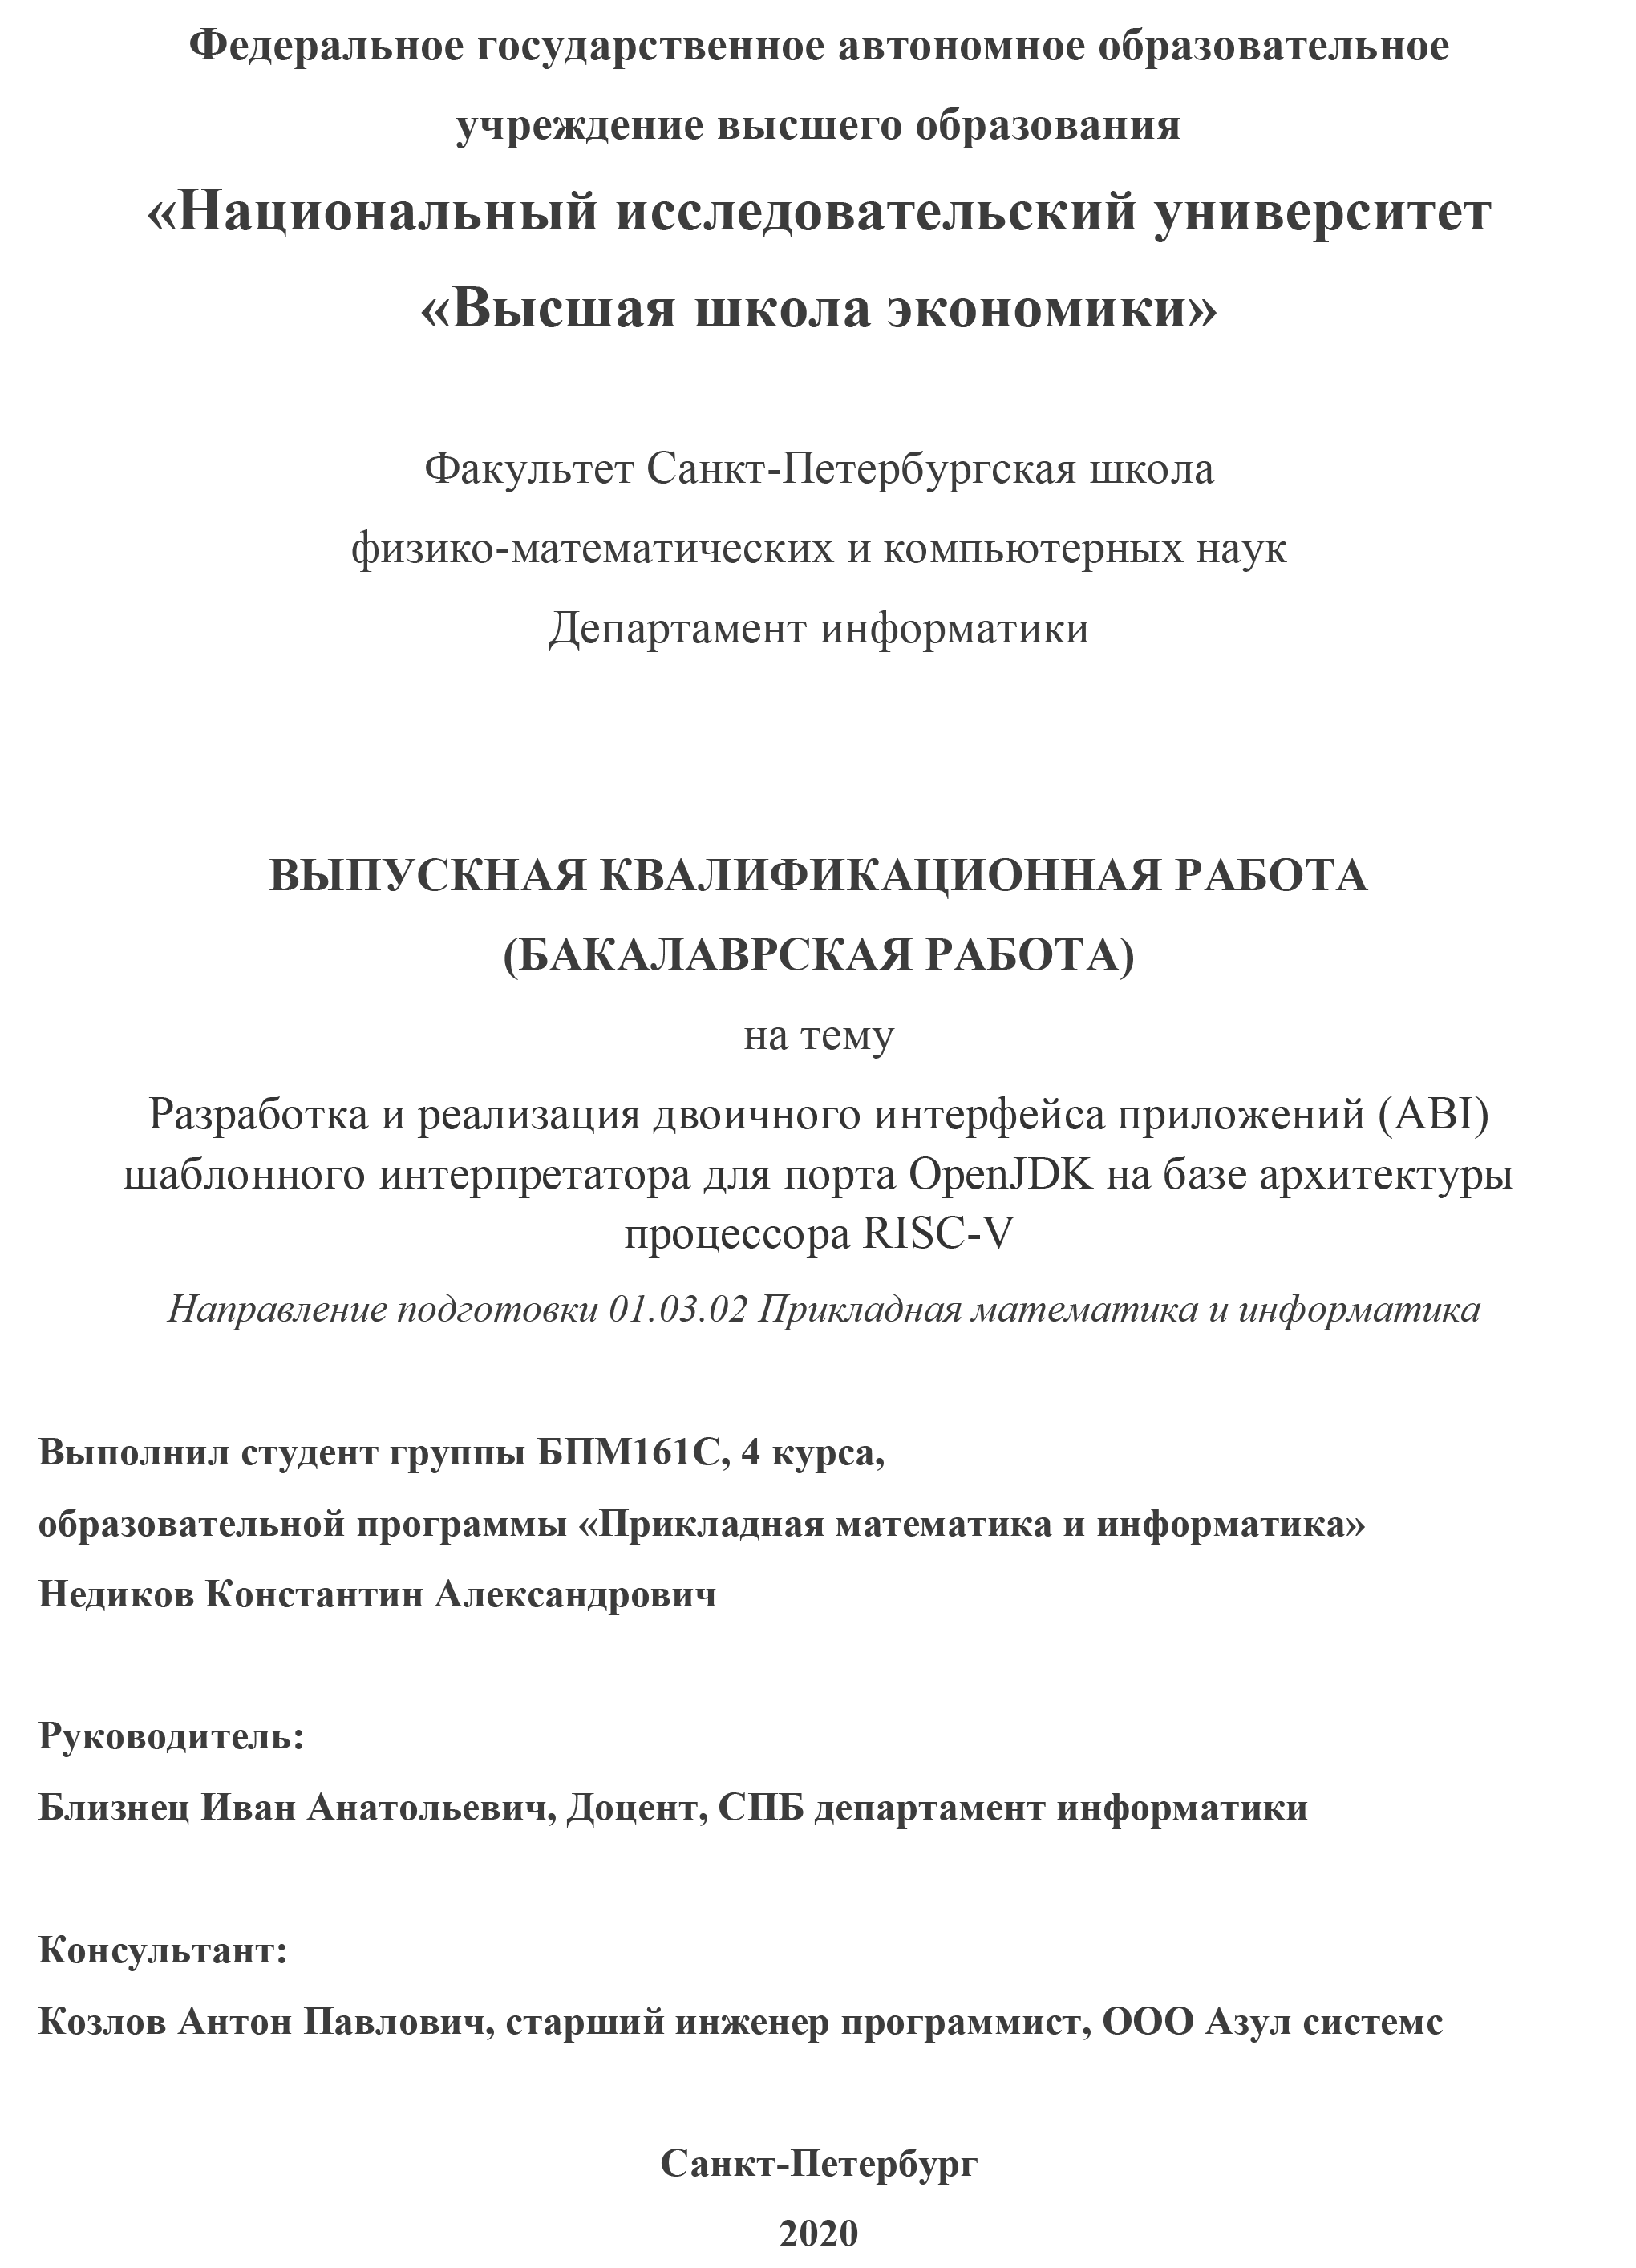
\includegraphics[scale=1]{figs/title.png}
\end{figure}

\newpage

\newgeometry{a4paper,top=20mm,bottom=20mm,left=30mm,right=15mm,nohead,includeheadfoot}
\setcounter{page}{1}

\tableofcontents

% У введения нет номера главы
\section*{Введение}
\renewcommand{\thefigure}{\arabic{figure}}
\subsection*{Актуальность и релевантные работы}

RISC-V --- это open-source архитектура процессора, которая с 2010 года разрабатывается для широкого круга применений. Данная разработка поддерживается многими крупными компаниями \cite{riscv:members}, в том числе такими как Alibaba, Google, Huawei, NVIDIA, Western Digital.

На текущий момент, платформа поддерживает исполнение множества программ и языков \cite{riscv:soft}, однако исполнение языка Java на RISC-V возможно только на двух исследовательских Java машинах, не подходящих для продуктовых решений из-за своей специфики и производительности.

OpenJDK --- это open-source проект, в котором разрабатывают эталонную \cite{openjdk_reference, openjdk:FAQ} продуктовую реализацию Java Development Kit (JDK), которая содержит Java Virtual Machine (JVM), библиотеку классов и прочие инструменты разработки, такие как компилятор javac. Имплементация JVM платформозависима, и её порты реализованы для многих современных архитектур \cite{openjdk:platforms}, но всё ещё нет порта для RISC-V.

\myfig{jvm.png}{Схематичное устройство JVM}{jvm}{0.6}

Упрощенное схематичное устройство JVM представлено на \figref{jvm}, сначала Java код компилируется в Bytecode инструкции (байткоды), которые попадают в JVM и там происходит их ассемблерная интерпретация в шаблонном интерпретаторе. Затем, когда статистика по исполнению будет собрана, активируется Just In Time (JIT) компилятор, оптимизирующий исполняемый код, однако периодически происходит деоптимизация кода, и исполнение снова возвращается в интерпретатор. Как видно, шаблонный интерпретатор --- ключевая и неотъемлемая часть JVM, наличие которой позволяет исполнять любой Java код.

При имплементации шаблонного интерпретатора необходимо продумать и реализовать его двоичный интерфейс приложения\footnote{Авторский перевод термина Application Binary Interface} (ABI), ключевую роль в котором занимают фреймы --- структуры данных, создаваемые на стеке при вызове функций. В Java фреймы содержат аргументы, локалы и прочие данные для интерпретации и выполнения ABI. Есть три ключевых перехода между функциями - из C в Java через входной фрейм, из Java в Java через Java фрейм и из Java в C через нативный Java фрейм.



\subsection*{Цель и задачи}

Данная работа ставит своей целью разработку и реализацию ABI шаблонного интерпретатора для порта OpenJDK на архитектуру процессора RISC-V. Для этого ставятся следующие задачи:

\begin{enumerate}
    \item Провести подготовительные работы для портирования OpenJDK, включающие в себя настройку рабочего окружения и реализацию базовых компонент порта OpenJDK.
    \item Разработать структуры фреймов и реализовать их для трех переходов между функциями в интерпретаторе.
    \item Определить набор данных, которые являются самыми востребованными в интерпретаторе и нуждаются в кэшировании в специально выбранных регистрах для уменьшения количества медленных обращений к памяти.
    \item Тестирование полученных результатов для проверки корректности реализации.
\end{enumerate}




\subsection*{Достигнутые результаты}

В рамках данной работы было сконфигурировано окружение, в том числе написаны различные скрипты для упрощения работы с ним, а также реализован генератор RISC-V ассемблера, необходимый для написания порта.

Были спроектированы структуры фреймов, основанные на нативном ABI C фреймов, что позволило сохранить единообразие системы, необходимое для корректной работы инструментов отладки и Runtime вызовов. Также входной, Java и нативный Java фреймы были реализованы в соответствии со всеми требованиями со стороны системы и нативных соглашений о вызовах. Их структура не подверглась значительным изменениям, в сравнении с другими портами портами, однако каждое решение по расположению данных на фрейме было обосновано.

Для выбора информации, нуждающейся в кэшированни, было проведено исследование с ручным и автоматическим сборами статистики, как для выявления полезности текущего кэширования данных, выбранного в других портах, так и для потенциального нахождения новых. Данные исследования показали острую необходимость кэширования ряда данных, в то время, как кэширование некоторых данных оказалось бесполезным или крайне сомнительным, требующем дальнейшего более индивидуального изучения. По ряду причин, включающих в себя большую трудозатратность, данное исследование не было полностью закончено и были намечены дальнейшие векторы развития в данном направлении, которые смогут помочь определить оптимальный набор данных для кэширования.

Для тестирования были выбраны несколько подходов, позволяющих, в первую очередь, проверить корректность работы с аргументами на фрейме, в том числе нативными, а также правильность создания и удаления фреймов со стека. Остальные аспекты данной работы не подлежат тщательному тестированию, поэтому их корректность была подтверждена лишь косвенно.

\subsection*{Структура работы}

В обзоре литературы представлены основные для данной работы источники информации в области как архитектуры RISC-V, так и проекта OpenJDK, а также рассмотрены альтернативы по замене литературы, необходимой для портирования OpenJDK.

В первой главе описаны работы по подготовке и настройке рабочего окружения, а также начало процесса портирования, а именно написание генератора ассемблера и неудачные попытки реализации вывода ошибок JVM.

Во второй главе представлены все факторы, учтенные в разработке фреймов, а также описание структур и реализации каждого фрейма.

В третьей главе представлены методы исследования по выбору информации для кэширования, а также полученные в ходе данного исследования результаты. 

В четвертой главе указаны используемые методы тестирования и представлены результаты по общей работе порта на данном этапе его разработки.

\renewcommand{\thefigure}{\arabic{section}.\arabic{figure}}

\section*{Аннотация}

Активно развивающаяся архитектура процессора RISC-V, имеющая большую поддержку от лидирующих компаний со всего мира, всё ещё не имеет реализации OpenJDK --- эталонной и эффективной среды для разработки и исполнения Java, одного из самых популярных языков программирования. Важнейшим элементом исполнения Java является шаблонный интерпретатор, для реализации которого необходимо разработать ABI, включающий в себя структуры фреймов на стеке и использование регистров для кэширования информации. В ходе данной работы были разработаны и реализованы структуры фреймов, основанные на нативном ABI фреймов RISC-V, также было проведено исследование, основанное на полуавтоматически собранной статистике исполнения Java кода, в результате которого были выявлены наиболее и наименее нуждающиеся в кэшировании данные. Также были найдены и использованы способы протестировать результаты на ещё неполностью рабочем порте.

\section*{Abstract}

The actively developing RISC-V instruction set architecture, which has great support from leading companies from around the world, still does not have an OpenJDK implementation --- a reference and efficient environment for developing and executing Java, which is one of the most popular programming languages. The most important element of Java execution is the template interpreter, for the implementation of which it is necessary to develop an ABI that includes stack frame structures and the use of registers for information caching. In the course of this work, frame structures based on the native ABI of RISC-V frames have been developed and implemented, as well as a study based on semi-automatically collected statistics on the execution of Java code, as a result of which the most and the least caching data have been identified. The solution has been found and used in testing the results on a still incomplete working port.

\section*{Обзор литературы}

\subsection*{Спецификация Java машины}

Главным и официальным источником информации о Java машине и её устройстве является The Java Virtual Machine Specification (JVMS)~\cite{jvms}. В нашей работе рассматривается тринадцатая версия JVMS, как самая актуальная на момент начала работы, однако интересующие нас разделы являются основополагающими и не менялись долгие годы. 
В разделе 2.3 JVMS описываются типы данных в Java, их размеры и строгая спецификация диапозона допустимых значений. Данный раздел крайне полезен при имплементации трансляции Java значений в значения языка C, и обратно, чтобы не нарушить спецификацию и внутреннее устройство этих языков. Раздел 2.6 является одним из самых основных для данный работы, так как описывает устройство Java фреймов, разработка которых является ключевым этапом в разработке ABI для \gls{порт}[а] Java машины. Фреймы создаются при каждом вызове метода, а текущим фреймом считается тот, что был создан при вызове текущего метода на исполнение. На фрейме хранятся аргументы, локалы, и стек вычислений, а также прочая информация, требуемая для реализации. Аргументы и локалы образуют единый список переменных функции и индексируются совместно таким образом, что если у нас имеется n аргументов и m локалов, то аргументы будут иметь индексы от 0 до n - 1, а локалы от n до n + m - 1, далее, при исполнении байткодов, логическая грань между переменными и локалами стирается, и всё обращение к ним происходит единообразно по индексу. Информация о количестве локалов, аргументов и размере стека вычислений рассчитывается во время компиляции, и содержится в структуре исполняемого метода.

Стоит отметить, что данная спецификация описывает требования, предъявляемые к системе, но не описывает детали имплементации, и тем более она не описывает устройство OpenJDK, понимание работы которого необходимо для его портирования.


\subsection*{OpenJDK}

Полной и качественной документации по внутреннему устройству OpenJDK не существует, однако весь код проекта находится в открытом доступе, частично задокументирован в виде комментариев к классам и методам, а остальную семантику выполнения процессов интерпретации можно вычитать напрямую из кода\cite{hotspot}.

Весь проект разделен на общую и платформозависимые части, которые относятся к конкретной операционной системе и процессору. Кодовая база проекта насчитывает сотни файлов в общей части, и десятки для каждой платформы, каждый файл может достигать нескольких тысяч строк в длину, что делает изучение всего проекта в короткие сроки маловозможным.

Большинство портов OpenJDK написаны на основе других, и по коду, или оставшимся от иной платформы комментариям, можно проследить данное заимствование, что, порой, может усложнять восприятие. Также встречаются редкие расхождения комментариев и имплементации, что так же сбивает с толку при прочтении. При анализе различных портом можно также заметить некоторые общие практики, относящиеся по большей части к организации кода и внутренних структур, и, наоборот, сугубо платформоспецифичные, которые уникальны и не поддаются общей характеристике.


\subsubsection*{Спецификация RISC-V}

Основным документом по работе с архитектурой RISC-V является его официальная спецификация~\cite{riscv:spec}, выложенная у них на сайте. В данном документе описаны кодировки и описания всех инструкций и регистров, а также специфику вычислений, внутренней работы и прочих аспектов, необходимых для разработчиков, пишущих низкоуровневые приложения под данную платформу. 

Остальную документацию по связанным с RISC-V окружением и компонентами можно найти на их официальной странице в GitHub~\cite{riscv:github}. Например, данная страница содержит репозиторий~\cite{riscv:convention}, в котором описана конвенция о вызовах~C, описывающая семантику выкладки аргументов в регистры и на стек при вызове C~функций. Также, на данной странице можно найти репозиторий~\cite{riscv:asm} с более подробной документацией некоторых ассемблерных особенностей данной платформы.


\subsection*{Выводы}

По данной тематике не удалось найти литературы, описывающей решение конкретной проблемы продумывания и имплементации ABI для OpenJDK, либо портирования OpenJDK на другие платформы, однако в данной среде есть немалое количество документов и спецификаций, посвященных системам, с которыми необходимо плотно работать. Необходимую литературу по OpenJDK можно заменить кодом и комментариями к нему, которые, однако, порой бывают невыверены или плохого качества. Остальная найденная литература по OpenJDK не имеет отношения к данному проекту прямым или косвенным образами, и потому не нуждается в упоминании.



\newpage
\safeoldsection[Подготовительные работы для портирования OpenJDK]{Подготовительные работы для\newline портирования OpenJDK}

Для разработки порта под другую платформу необходимо сделать некоторые предварительные шаги для инициализации всей работы. Этот этап разработки выполнялся совместно, в команде из 4 человек. 
Далее, на протяжении данной главы, о задачах, выполненных индивидуально, будет оговариваться отдельно.

% \TODO{ возможный перефраз: Далее, на протяжении данной главы, будут делаться уточнения, если задача выполнялась индивидуально.}



\subsection[Настройка обеспечения для разработки на базе RISC-V]{Настройка обеспечения для разработки\newline на базе RISC-V}

Процессоры, произведенные на базе архитектуры RISC-V ещё не поступили в массовое производство, а тестовые образцы поставляются в очень ограниченном количестве и приобрести их проблематично из-за высокого спроса на рынке. В связи с этой проблемой единственным доступным способом является разработка на эмуляторе RISC-V, способным запустить операционную систему.

Был найден QEMU эмулятор RISC-V \cite{riscv:qemu}, который ещё находится в разработке, но уже способен запускать linux и работать безошибочно для большинства задач, а также выбран RISC-V GNU toolchain \cite{riscv:gnu}, содержащий необходимые инструменты разработки для кросс-компиляции\footnote{Компиляции кода на платформу, отличную от той, на которой запущен кросс-компилятор} и отладки \cpp кода на RISC-V. Были написаны docker\footnote{Программа для удобной контейнеризации и развертки программных сред} образы для более удобной командной разработки и переносимости настроенного окружения. Также были написаны скрипты для упрощенного запуска данных образов с монтированием директорий и настройкой всех необходимых параметров.

Для отладки был использован GDB из RISC-V GNU toolchain, который работал с кодом, выполняющимся на QEMU, посредством клиент-серверного взаимодействия, так как возможностей GDB, реализованного на RISC-V, не хватало для тщательной отладки. Однако, подобное взаимодействие усложнило настройку GDB, поэтому были написаны специальные скрипты для запуска сервера и клиента с различными флагами, а также подключением отладочных символов проекта.
    
    
\subsection{Настройка OpenJDK}

Для проверки корректности настроенного окружения было решено запустить zero порт OpenJDK, который написан на \cpp и является почти полностью кроссплатформенным, однако для его запуска было необходимо избавиться от ошибок компиляции, возникающих в платформозависимых вставках в общей для всех портов части кода. В итоге, zero порт успешно запустился на эмуляторе RISC-V, и инициализация Java машины на нём занимала около двух минут, что демонстрирует низкую производительность QEMU и zero порта.

% \TODO{Стоит ли писать про настройку индексации в Clion?}
% Также мы смогли настроить clion для работы с OpenJDK и её корректной индексации, что, в целом, не предполагается разработчиками Java

Ради ускорения разработки мы выбрали стандартный метод портирования, заключающийся в копировании исходного кода некого порта и его постепенном переписывании. Для данной цели решено было выбрать порт PowerPC, так как его код показался чище, а архитектура ближе к RISC-V, чем другие. Тем не менее, данный выбор не является критичным или ключевым, и был сделан, по большей части, из соображений удобства, а при решении некоторых задач мы смотрели на реализацию других портов OpenJDK.

Прежде чем приступить к платформозависимой реализации интерпретатора, были устранены ошибки компиляции, вызванные копированием другого порта, а также настроить некоторые платформозависимые части общего для всех портов кода.


\subsection{Реализация базовой функциональности порта}

Процесс интерпретации происходит с помощью ассемблерного кода, генерирующегося при инициализации JVM. В общей части OpenJDK реализован фреймворк, с помощью которого можно написать свой генератор ассемблерного кода. Для этого были воссозданы все правила генерации кодов инструкций, описанные в спецификации RISC-V, и таким образом генератор был реализован. 

В OpenJDK реализован код, который печатает файл с ошибками и состоянием системы при исключительных ситуациях и экстренном выходе из программы. Основная часть данной реализации зависит одновременно от операционной системы и архитектуры процессора. Было решено написать эту часть и для нашего порта, что помогло бы ускорить нахождение ошибок, возникающих при написании системы, эта задача выполнялась индивидуально. Однако, из-за неизвестной ошибки в эмуляторе, значение всех регистров портилось при обработке ошибок на процессоре. Данное поведение помешало разработке, и процесс был остановлен на полпути. Позднее, разработчики QEMU исправили данную ошибку в своей новой версии, однако данная часть так и осталась нереализованной в связи с более важными возникающими задачи.


\subsection{Выводы}

В качестве системы исполнения кода был выбран эмулятор QEMU, а для компиляции и отладки кода был выбран RISC-V GNU toolchain, и всё это было положено в docker образы для удобной дальнейшей работы. Окружение было успешно настроено, что было проверено запуском zero порта. Для процесса портирования был выбран PowerPC порт в качестве основы для реализации, также был написан генератор ассемблерного кода RISC-V, и предпринята попытка реализации кода, отвечающего за печать ошибок виртуальной машины, которая оказалось неуспешной из-за ошибки в QEMU.




\section{Разработка и реализация фреймов}

Структуры \gls{фрейм}[ов] в OpenJDK являются ключевым элементом ABI всего интерпретатора и определяют такие вещи, как выбор и способ сохранения необходимой информации во время \glslink{интерпретация}{интерпретации} \gls{метод}[ов]; способ взаимодействия Java \gls{метод}[ов], как друг с другом, так и с JNI и Runtime \gls{метод}[ами], вызываемыми в процессе интерпретации; семантику взаимодействия со стеком вычислений, локальными значениями и аргументами. Правильное создание данных структур должно опираться как на нативную реализацию структуры \gls{фрейм}[ов], чтобы сохранить совместимость с нативными вызовами и инструментами отладки, так и на создание и использование этих структур в интерпретации, чтобы обеспечить максимально быструю работу приложения.


\subsection{Разработка структуры фреймов}

Первой задачей разработки структуры \gls{фрейм}[ов] было нахождение или составление описания нативных \gls{фрейм}[ов] для языка C. Данные, найденные в онлайн лекции Parallel \& Distributed Operating Systems Group~\cite{lecture:frames}, не являются официальным документом от разработчиков компилятора языка~C, поэтому их необходимо было проверить, для чего использовался \gls{метод} обратной инженерии. Были написаны различные программы на языке C, в которых были отражены ключевые сценарии вызовов \gls{метод}[ов], передачи аргументов и работы с локальными переменными. Далее, данный код был скомпилирован с помощью RISC-V GNU GCC~\cite{riscv:gnu} компилятора в ассемблерный код RISC-V, после чего в нём были выявлены места, отвечающие за создание и заполнение \gls{фрейм}[ов]. Семантика данного кода полностью соответствовала найденной структуре, и было принято решение использовать её в качестве основы для создания структуры Java \gls{фрейм}[ов]. 

Проектирование структуры Java \gls{фрейм}[ов] для RISC-V было основано на структуре \gls{фрейм}[ов] для архитектуры PowerPC, однако своё влияние на разработку оказали существенные различия в нативных \gls{фрейм}[ах] данных архитектур, а именно: нативный ABI RISC-V \gls{фрейм}[ов] содержит только адрес в памяти, указывающий на начало \textbf{предыдущего} \gls{фрейм}[а](началом \gls{фрейм}[а] будем считать последний байт перед этим фреймом), и адрес возврата для \textbf{текущей} функции, в то время как у PowerPC хранится начало \textbf{текущего} \gls{фрейм}[а], адрес возврата \textbf{вызываемой} функции, имеется зарезервированное место под первые 8 аргументов и все эти значения лежат внизу \gls{фрейм}[а], а не наверху, как в RISC-V.
Данные отличия, а также наличие регистра fp\footnote{Образовано от frame pointer}, указывающего начало текущего \gls{фрейм}[а], повлекли изменения в реализации \gls{метод}[ов], которые помогают осуществить просмотр данных \gls{фрейм}[а] и навигацию между \gls{фрейм}[ами] во время исполнения внутренних Runtime вызовов.

    Одной из особенностей архитектуры RISC-V является обязательное выравнивание вниз на 16 байт значения в регистре sp\footnote{Образовано от stack pointer}, которое должно указывать на последний байт текущего \gls{фрейм}[а]. Во время исполнения кода необходимо соблюдать данное выравнивание, что означает выбор одного из трех решений:
\begin{enumerate}
    \item Применять выравнивание ко всем данным, выкладываемым на стек.
    \item Помнить невыровненное смещение относительно sp, при работе со стеком сдвигать и его, и значение в sp.
    \item Создавать \gls{фрейм} фиксированного размера и выкладывать все данные внутри него.
\end{enumerate}

Первый вариант нам не подходит из-за того, что размер данных на стеке увеличится примерно в 2 раза, что является неоправданной тратой памяти. Решено было выбрать третий, так как, хоть он и требует небольших накладных расходов памяти на поддержание места под значения, которые не всегда необходимо сохранять в памяти, однако, в отличие от второго, он не усложняет работу со значениями на стеке, что может существенно замедлить процесс интерпретации.
% TODO написать про то, что остальные поля заполнялись и менялись исходя из нуждн реализации
% TODO вставить ссылку на приложения со структурой фрейма

\subsection{Реализация входного фрейма}

Самой первой точкой входа в интерпретатор является генерация входного \gls{фрейм}[а], который, как и все остальные \gls{фрейм}[ы], написан с помощью нашего ассемблерного генератора. 

Для создания входного \gls{фрейм}[а] необходимо рассчитать и выделить под него место на стеке и заполнить все структуры, отображенные на \figref{входной_фрейм}, актуальными данными. Для заполнения нативного ABI необходимо сохранить в верхние два слова значения регистров ra\footnote{Образовано от return adress} и fp, которые указывают на адрес возврата функции и на начало предыдущего \gls{фрейм}[а] соответственно. "Сохраненные регистры" содержат в себе значения всех неизменяемых регистров, кроме fp и sp, это необходимо для соблюдения конвенции о вызовах~C~\cite{riscv:convention}, а именно, соблюдение правила о том, что неизменяемые регистры должны иметь одно и то же значение до и после вызова функции. Значение sp регистра будет сохранено в регистре fp, а значение fp мы сохранили в нативном ABI, поэтому их значения не нужно сохранять дополнительно. Локальные данные содержат несколько значений, доступ к которым может потребоваться во время интерпретации, а исходящие аргументы - это аргументы, пришедшие из C вызова, которые необходимо перекопировать на стек для совместимости разных вызовов.
 
\myfig{entry_frame.png}{Структура входного фрейма}{входной_фрейм}{0.5}
 
Во время заполнения данных структур возникали трудности с расставлением правильных смещений относительно fp регистра для точного определения начала структур. Также было необходимо правильно выбрать регистры для всех промежуточных расчетов, чтобы не получилось перекрытия данных. Помимо этого, на данном этапе появилась необходимость загрузки констант в регистры, так как архитектура RISC-V не предусматривает загрузку 64-битной константы в регистр одной инструкцией, и для этих целей нужно написать свой генератор, который по константе сгенерирует оптимальный набор инструкций, загружающих в регистр эту константу. Данный генератор уже написан в GCC, однако найти этот код в огромной системе не получилось, поэтому был написан собственный.

\TODO{Нужно ли писать более точные технические подробности про генератор?}

\TODO{Нужно ли указать, что генератор писался коллективно?}



\subsection{Реализация Java фрейма}
При вызове Java \gls{метод}[а] происходит создание Java \gls{фрейм}[а]. На предыдущем \gls{фрейм}[е] должны быть выложены аргументы, а регистр s7, который мы выбрали и назвали esp\footnote{Образовано от expression stack pointer}, и который указывает на первый свободный слот стека вычислений\footnote{Авторский перевод термина operand stack из JVMS}, указывает на место, куда необходимо выложить локалы. В зависимости от размера стека вычислений предыдущего \gls{фрейм}[а], занятого на нём места и количества аргументов и локалов текущего \gls{метод}[а], предыдущий \gls{фрейм} необходимо увеличить, чтобы вместились все данные, либо уменьшить, чтобы не занимать лишнего места на стеке, которое мы не будем использовать во время интерпретации текущего \gls{метод}[а], для этого нужно соответствующим образом сдвинуть регистр, указывающий на начало текущего \gls{фрейм}[а], запомнив конец предыдущего \gls{фрейм}[а] до смещения в специально отведенном месте на стеке, чтобы восстановить его первозданный вид после выхода из \gls{метод}[а].

Трудности в данной работе возникали, как и для входного \gls{фрейм}[а], в правильном расчете всех размеров и сдвигов. В отличие порта PowerPC, у нас нет необходимости перекопировать структуры нативного ABI при изменениях родительского \gls{фрейм}[а], а также у нас нет необходимости хранить на последнем \gls{фрейм}[е] место под 8 аргументов для Runtime вызовов. Данные отличия помогли изменить структуру расчетов размеров \gls{фрейм}[ов], сделав её проще и понятнее для восприятия, не жертвуя количеством инструкций, необходимых для этих расчетов.

\myfig{Ijava_frame.png}{Структура Java фрейма}{java_фрейм}{0.45}

Были предприняты попытки по значительному изменению структуры Java \gls{фрейм}[а], изображенного на \figref{java_фрейм}, однако они не увенчались успехом. Для упрощения обращения к аргументам и локалам \gls{метод}[а], которые находятся на предыдущем \gls{фрейм}[е], можно зарезервировать регистр, который будет указывать на начало этих данных. Однако можно заметить, что эти данные расположение прямо перед началом текущего \gls{фрейм}[а], таким образом, что регистр fp указывает на конец этих данных с учтенным смещением на 16 байт. Если полностью инвертировать порядок аргументов и локалов, то можно добиться того, чтобы первый fp указывал ровно на первый аргумент, и от него можно было бы получить доступ ко всем остальным, однако, в связи со спецификацией Java, аргументы выкладываются на стек с помощью обычных байткодов, выкладывающих любые значения на стек, что делает невозможным контроль данного процесса. Единственным возможным решением в данном случае является копирование аргументов в обратном порядке на новое место при вызове \gls{метод}[а], однако это слишком дорогая операция по количеству инструкций на обращение к стеку, и, в итоге, более правильным, в целях оптимизации, решением будет выделение дополнительного регистра для упрощения адресации.

Также были предприняты попытки изменить расположение мониторов\footnote{Специальные структуры, отвечающие за механизмы синхронизации многопоточных вычислений}, в связи с тем, что исходя из статических данных, полученных из Java компилятора, нельзя вычислить точное количество места, требуемого под расположение мониторов, что приводит к копированию всех данных под мониторами, при выкладывании их на стек и сопутствующим расширении \gls{фрейм}[а]. Исходя из данных рассуждений следует вывод, что необходимо располагать мониторы как можно ближе к концу \gls{фрейм}[а], чтобы как можно меньше данных пришлось копировать. При рассмотрении рисунка \ref{fig:java_фрейм}, следовательно, можно заметить, что передвигать мониторы на первую или вторую позицию будет менее рационально с позиции уменьшения количества копируемых данных. Исходящих аргументов и локалов на \gls{фрейм}[е] при выкладывании монитора ещё нет, в связи с тем, что мониторы выкладываются только на текущий фрейм, а значит остаются только позиции до или после стека вычислений, однако, исходя из того, что размер стека вычислений не учитывает количество локалов вызываемых \gls{метод}[ов], по причине невозможности данных подсчетов, при выкладывании мониторов после стека вычислений мы не только лишимся возможности быстрого изменения размера стека при вызове, чтобы занять свободное место стека вычислений, но и разорвем непрерывность аргументов и локалов на стеке, что увеличит количество операций, требуемых на работу с ними. Таким образом, в особенности учитывая тот факт, что мониторы выкладываются преимущественно при пустом стеке вычислений, их текущая позиция является оптимальной.



\subsection{Реализация нативного Java фрейма}
JNI \gls{метод}ы написаны на языках C или \cpp и для их вызова необходимо соблюдать конвенцию о вызовах C. Для решения этой задачи создается специальная структура нативного Java \gls{фрейм}[а], отличающаяся от своей ненативной реализации отсутствием стека вычислений и нативным форматом исходящих аргументов. Данный \gls{фрейм} является лишь прослойкой между Java и С языками, служащий лишь в качестве корректного форматирования аргументов, выкладывании монитора для синхронизированных вызовов и сохранением необходимых данных в структуре ijava\_state.


\myfig{native_frame.png}{Структура нативного Java фрейма}{нативный_java_фрейм}{0.6}


В OpenJDK копирование Java аргументов в C формат представлено двумя способами - быстрым и медленным. Данный выбор переключается с помощью выставления специального флага при запуске JVM, которая по умолчанию использует быструю реализацию. Медленное копирование аргументов читает сигнатуру \gls{метод}а непосредственно в ассемблерном коде, и по ней происходит копирование каждого типа данных из сигнатуры надлежащим образом. Данный \gls{метод} позволяет сгенерировать код один раз для всех вызовов \gls{метод}а, однако чтение и разбор сигнатуры из ассемблера накладывает дополнительные вычислительные затраты на данный код, а также требуют двух Runtime вызовов для взятия необходимых значений из \gls{метод}а. Быстрое копирование аргументов подразумевает генерацию уникального кода для каждой сигнатуры, который будет максимально быстро копировать аргументы, зная про формат сигнатуры на момент генерации. В рамках данной работы было реализовано оба этих \gls{метод}а.

В процессе генерации нативного Java \gls{фрейм}[а] делается значительно больше проверок и обработок исключительных ситуаций, чем при генерации ненативного \gls{фрейм}[а]. Помимо этого, появляется необходимость обработки результата JNI \gls{метод}а, чтобы он соответствовал значениям Java типов, специфицированных в JVMS. Так, например, значения булевого\footnote{Тип данных, имеющий только два значения - ложь и истина} типа в Java должны содержать только $0$ или $1$, что является ложью или истиной соответственно, в то время как в спецификации C указано, что $0$ соответствует ложному значению, а любое другое число истинному. В связи с подобными ограничениями были придуманы и реализованы минимальные по сложности инструкции переводов значений C типов в значения, удовлетворяющие Java спецификации и внутренней работе порта.

\TODO{Ссылки на код в приложении? Объяснение примера с булевым значением?}

\subsection{Выводы}

В глобальную структуру фреймов не удалось привнести ничего кардинально нового, однако каждое принятое решение по структуре было обдумано и обосновано. Особенности платформы RISC-V были корректно учтены при проектировании фреймов, что отразилось в фиксированном размере каждого фрейма, нативном ABI, копировании нативных аргументов и прочем. Реализация генерации данных структур, их заполнении и поддержки была сделана с учетом необходимости высокой скорости работы приложения, что выражается в экономии количества вызванных инструкций.


\newpage
\safeoldsection[Кэширование информации интерпретатора]{Кэширование информации\newline интерпретатора}

Обращение к памяти на стеке для чтения или записи является долгой операцией, поэтому мы хотим уменьшить количество таких обращений. В процессе работы интерпретатора нам нужно часто обращаться к одним и тем же данным, которые лежат где-то в памяти, и такие данные (или адреса, указывающие на них) можно положить в специальные регистры, значения в которых не будут портиться при вызовах C функций, так как по общему соглашению значения этих регистров должно быть одинаковым до и после вызова функции, а потому их называют неизменяемыми.

Всего в архитектуре RISC-V 12 неизменяемых регистров, один из которых используется, как fp регистр. В итоге получается 11 регистров, которые мы можем использовать под свои нужды. На каждой архитектуре разное количество этих регистров, на PowerPC их 18, и нам не хватает регистров, чтобы закэшировать всю информацию, что кэшируется в PowerPC, а потому было решено провести исследование со сбором статистики использования данных регистров, чтобы выбрать наиболее необходимые.



\subsection{Выбор источников для сбора статистики}

Сбор статистики должен производиться из объективных источников, чтобы реальные пользователи OpenJDK смогли ощутить схожий с нашими данными прирост производительности. Таким образом, было выбрано 3 основных источника.
Первый - инициализация JVM, которая происходит при каждом запуске Java приложений, и, что не менее важно, основная его работа происходит без использования JIT компиляции, что делает данные замеры ещё более объективными.
Второй источник - Renaissance Suite \cite{renaissance}, тест производительности, основанный на реальных приложениях, использующий в своих тестах библиотеки scala, spark и прочие жизненные примеры использования JVM, данный тест является новым, объемным и широко распространенным.
Третий источник - SPECjvm2008, это первый, популярный в свое время, тест производительности Java, основанный на реальных приложениях.

Одной из задач данной работы было создание универсальных полуавтоматических инструментов, позволяющих получать данные из любых источников, что могло бы значительно ускорить работу по корректировке и перепроверке результатов, поэтому рассмотренные источники могут быть дополнены в будущем, а цель текущего их выбора состоит в базовой проверке гипотез и получения начальных объективных, но не обязательно полных, данных. 



\subsection{Ручной сбор статистики}

Первой идей сбора данных был ручной подсчет использования регистров в байткодах, а далее, используя статистику по количеству исполненных байткодов, собранных с помощью инструментов OpenJDK, можно было бы получить общую статистику по количеству использования регистров в порте. Целью данного сбора было выявление сильноиспользуемых и малоиспользуемых регистров, которые уже кэширует информацию в PowerPC порте, и, в большинстве своем, в RISC-V. Данные собирались по ещё недописанному порту RISC-V, однако, на момент сбора статистики, в нём было реализовано уже порядка 80 процентов байткодов, остальные же брались с PowerPC из предположения, что используемые данные на разных портах не сильно различаются.

В итоге мы хотели получить количество обращений к памяти к каждому полю, если бы оно не было закэшировано, что означает, что простым подсчетом количества использований обойтись не получится, так как можно загрузить данные во временный регистр один раз и потом обращаться к ним много раз во время интерпретации байткода. Автоматический сбор таких данных тоже маловозможен, преимущественно из-за очень сложной интерпретации измененния данных. Автоматически нельзя понять, после каких изменений данные необходимо записать в память, а какие изменения можно расчитывать во временных регистрах. Также все временные регистры теряют информацию после каждого Runtime вызова, что тоже усложняет расчеты. В дополнение к этому, иногда можно изменить сигнатуру некоторых функций, что позволит передавать значения регистров внутрь и избавит от лишнего взятия этих данных внутри функции, если было необходимо взять их ещё и снаружи. И что не менее существенно, целью было произвести подсчет для порта RISC-V, а он ещё находится в состоянии разработки, и не может полностью обработать вычисления из выбранных источников. 

Все наложенные ограничения привели к необходимости производить подсчет вручную, а именно, посчитать приближенное количество загрузок и сохранения данных для каждого значения, если бы оно не было сохранено в регистр. Данная информация была подсчитана для каждого из 128 методов, и всех методов, вызываемых в процессе их исполнения, которые обеспечивают работу 251 байткода. Все полученные результаты были занесены в таблицу, а также были настроены формулы по автоматическому пересчету значений, позволяющие в конечном счете загрузить в таблицы статистику по исполнению байткодов и автоматически получить статистику по использованию данных.

Данный подсчет не учитывает код, вызываемый на момент создания фреймов, или же код, переключающий байткоды, потому что эти данные сложнее получить без существенных модификаций порта x86\_64, на котором осуществлялся сбор статистики по исполнению байткодов, из расчета на то, что Java компилируется в одинаковый набор байткодов на каждой платформе. Однако некоторые изменения пришлось внести в связи с тем, что счетчики байткодов переполнялись при анализе Renaissance Suite, поэтому необходимо было сделать модификации для подсчета статистики в 64-битных значениях.



\subsection{Автоматический сбор статистики}

После проведения ручного сбора статистики захотелось провести более подробный анализ данных, чтобы посчитать не только использование уже закэшированных данных, но и данных, которые потенциально можно было бы закэшировать. Поскольку мы не знали заранее всех данных, которые хотим посчитать, а также нам хотелось бы иметь возможность не учитывать какие-то данные, либо добавлять новые по ходу исследования, то ручной сбор уже не подходил, но и проблемы автоматического не исчезли. Идеальной архитектурой для данного сбора был бы порт, у которого было бы бесконечное количество временных регистров, и ни одного неизменяемого, чтобы каждый раз обращение к данным происходило через память, но чтобы данные сохранялись во временных регистрах и использовались через них, пока это возможно. Такого порта не существует, однако архитектура x86\_64 наиболее близка к подобному, и имея посчитанную вручную статистику для немногих закэшированных на ней данных, можно было бы собрать автоматическую статистику на всех остальных. 

Данный подход потребовал переписать сотни обращений к памяти, проинструментировать их для сбора статистики, что оказалось долгой и неприятной задачей. Также мы столкнулись с проблемой интерпретации получаемых данных, так как все хитрые зависимости и условности при использовании данных, которые были посчитаны вручную, теперь не работали и необходимо было учитывать их как-то автоматически, что сделать полностью было невозможно. Из-за сильной иерархичности доступа к данным была добавлена возможность вести подсчет без учета доставаемых предков в иерархии доступа, например, если в структуре method лежит структура constMethod, а в ней cachePool, то, при загрузке всех трех полей последовательно, в статистике будет учтена только загрузка cachePool. Подобные усложнения помогли избавиться от некоторых проблем с интерпретацией данных, однако породили сильные зависимости между собранными данными и усложнили общий подход к их интерпретации. Также не получилось полностью учесть весь контекст, и для интерпретации данных периодически необходимо анализировать код, чтобы их понять, например, если мы загружаем три разных поля из структуры constMethod примерно одинаковое количество раз, мы не можем без анализа кода сказать, нужно ли нам все эти три раза было грузить constMethod, или они все грузятся после того, как constMethod был загружен в другой временный регистр. Ещё большую путаницу вводит то, что на x86\_64 количество временных регистров не бесконечно и сильно меньше, чем у RISC-V, поэтому периодически данные грузятся по несколько раз, где в RISC-V можно было бы загружать их только один.

Все перечисленные факторы существенно замедлили процесс анализа данных, что, в совокупности с общим объемом работы и возникающими непредвиденными трудностями в процессе инструментирования обращений, не позволило провести расчеты для всех данных, использующихся в порте. Часть данных была выбрана из соображений проверки ручного сбора данных, остальные были выбраны из представления о частоте их использования по количеству их встречаемости в коде.



\subsection{Обработка результатов}

Для обработки результатов с первого метода были использованы флаги OpenJDK \textit{PrintBytecodeHistogram} и \textit{ActiveProcessorCount=1}, чтобы распечатать статистику по выполненным байткодам и сделать исполнение кода на одном процессе, иначе подсчет статистики будет собираться некорректно. Для запуска Renaissance Suite использовались параметры \textit{\texttt{--}functional\texttt{-}test \texttt{-}r 1 all}, а для SPECjvm2008 \textit{\texttt{-}mi 1 \texttt{-}ma 1 \texttt{-}bt 1 \texttt{-}ikv}.

Всего в инициализации JVM было исполнено 48 миллионов байткодов, в Renaissance Suite 225.7 миллиардов, а в SPECjvm2008 628.7 миллионов. По данным ручного сбора, распределения по использованию данных (в процентах от их общего числа) при инициализации JVM и в Renaissance Suite близки друг к другу, в SPECjvm2008 ситуация отличается некритично, там выше процент использования локалов и указателя на байткод, что обусловлено большим процентом математических и околоматематических байткодов, которые много оперируют со стеком и данным указателем.

С помощью автоматического тестирования удалось найти и исправить некоторые ошибки ручного тестирования, после исправления которых мы видим данный результат на инициализации VM: регистры указателя на байткод (bcp), текущего потока (threads), локалов (locals), верхушки стека вычислений (TOS) и начала фрейма (fp) используются десятки миллионов раз. Автоматически собранная статиста показывает, что таблица диспетчеризации (dispatch\_table) используется 48 миллионов раз, в ручном сборе она используется ноль раз, ибо отрабатывает только в исключительных случаях, которые не учитывались. Данная разница просто объясняется тем, что данное значение используется при переходе между байткодами и не учитывается в ручном подсчете. Также в ручном подсчете не полностью учитывается указатель на стек вычислений (esp), 7 миллионов в ручном сборе и более 58 при автоматическом. Данное отличие обусловлено изменением данного показателя между байткодами, а из-за частой изменяемости значения, при каждом обращении нужно делать и загрузку, и сохранение в память, что удваивает количество обращений к памяти. Указатель на конец предыдущего фрейма (sender\_sp) используется только при возврате из метода, которых было около 2.5 миллионов, и надобность в данном кэшировании минимальна. Регистр таблицы содержания (TOC) в шаблонном интерпретаторе не используется в принципе, он нужен только для JIT компиляции, а значит можно в будущем заменить его на регистр, не использующийся в JIT компиляции, например locals. Регистр мониторов (monitors) показывает также крайне низкие показатели - почти 6 тысяч в ручном тестировании и 112 в автоматическом. Данная разница сильно проявляется из-за неучтенных в ручном тестировании вызовов синхронизированных методов, которые прибавляют 106 тысяч использований. Данный регистр является самым неоднозначным из всех вышеперечисленных, так как его использование очень сильно зависит от специфики приложений, и в будущем необходимо найти программу с преобладающими параллельными вычислениями, чтобы собрать данные и посмотреть на реальное использование данного регистра. Если даже в параллельной среде этот регистр задействован слабо, то можно избавиться от его кэширования, но если же он проявляет свою необходимость в данных приложениях, то стоит его оставить для большей универсальности OpenJDK порта. Остались регистры с кэшем хранилища констант (const\_pool) и метода (method), которые используются по 6-7 миллионов раз, если сопоставить ручную и автоматическую статистики. Данные показатели не очень высокие, но пока им не нашлось достойной замены.

Автоматический сбор успешно справился с задачей проверки и уточнения ручного сбора статистики, однако, несмотря на вдвое большее количество рассмотренных данных, более удачных кандидатов на кэширование ещё не удалось выявить. Также не были рассмотрены регистры, необходимые для кэширования данных, помогающих облегчить отладочные сборки, профилирование OpenJDK, а также прочих побочных путей исполнения, в связи с тем, что в этих задачах скорость исполнения не является приоритетной ценностью, и ей можно пожертвовать при необходимости. 


\subsection{Выводы}

Были разработаны две методики сбора данных, которые отлично показали себя именно в совокупном использовании. Незначительные отличия в данных с выбранных источников показывают их объективность. В результате удалось выяснить крайнюю важность таких регистров, как bcp, TOS, esp, threads, locals, fp и dispatch\_table. Также свою полезность продемонстрировало кэширование method и const\_pool. Если monitors и sender\_sp показали весьма сомнительные результаты, и потенциально от них можно избавиться, то от кэширования TOC в интерпретаторе нет никакой пользы, его можно кэшировать его только при входе в JIT компиляцию, если это технически возможно.

Данное исследование оказалось более трудоемким, чем изначально предполагалось, что, в итоге, повлияло на его неполноту и незаконченность некоторых результатов. Однако уже на данном этапе были сделаны выводы относительно использования, либо потенциального использования регистров в RISC-V порте, что так или иначе будет учтено при его дальнейшей разработке. Также интересным бонусным результатом был вывод о том, что можно ускорить порт PowerPC, добавив в него отсутствующее кэширование fp регистра, что можно сделать, использовав ещё незадействованный регистр, либо же заменив на него sender\_sp.

Потенциальным продолжением данного исследования может быть задействование изменяющихся регистров в качестве кэшируемых, при сохранении их на стек при каждом Runtime вызове. Подобное исследование завязано не только на полной статистике по использованию данных, но и на полном анализе использования изменяемых регистров в коде, количество которых также весьма ограничено. 


\section{Тестирование результатов}

\subsection{Проблематика и направленность тестирования}

\subsection{Этапы тестирования}



% У заключения нет номера главы
\section*{Заключение}

Главным результатом данной работы является реализация разработанного ABI шаблонного интерпретатора для порта OpenJDK на архитектуру процессора RISC-V. В рамках выполнения поставленной цели были достигнуты следующие задачи:

\begin{enumerate}
    \item Были настроены GNU Toolchain и QEMU эмулятор RISC-V, позволяющие компилировать и запускать проект с помощью специально написанных для этого скриптов, упрощающих всё взаимодействие. Успешность настроенного окружения была проверена посредством запуска zero порта OpenJDK. Был написан генератор RISC-V ассемблера, однако из-за неполадок в QEMU не удалось реализовать печать ошибок JVM.
    
    \item При проектировании фреймов были учтены все особенности платформы RISC-V и её нативный ABI, и хоть глобальная структура не изменилась кардинально в сравнении с другими портами, однако каждое решение было принято обосновано. Реализация генерации фреймов, их заполнении и поддержки была сделана с учетом необходимости высокой скорости работы приложения.
    
    \item Были разработаны ручная и автоматическая методики данных, которые были применены к трем источникам - инициализации JVM, Renaissance Suite и SPECjvm2008. Наиболее полезными оказались кэширующие регистры bcp, TOS, esp, threads, locals, fp и dispatch\_table. Регистр sender\_sp оказался малополезным, а TOC вовсе неиспользуемым, и от них необходимо избавиться, по мере технической возможности. Для проверки полезности monitors было получено недостаточно данных, поэтому необходимо углубить данное исследование в будущем. Кандидатов на замену данным регистрам также не удалось обнаружить, поэтому необходимо произвести более тщательное исследование.
    
    \item Несмотря на трудность тестирования нерабочего порта OpenJDK, было успешно сгенерировано и пройдено 1289 тестов на различные сигнатуры методов и передачу параметров. Генератор случайных арифметических выражений позволил протестировать работу с локалами. Рабочая часть инициализации Java также доказывает корректность произведенной работы.
\end{enumerate}

В качестве дальнейшей работы над проектом могут быть расширение и углубление исследования кэширования информации, которое позволит ответить на неразрешенные вопросы о полезности кэширования мониторов и нахождении замены иного малополезного кэширования. Также остались нереализованными процессы, вызываемые при создании фреймов, необходимые для профилирования и продвинутого сбора статистики исполнения. Общая структура ijava\_state, широко используемая в Runtime вызовах, одновременно содержит информацию, необходимую только в нативных фреймах, а также необходимую только в ненативных, что может быть соптимизировано, если тщательно проанализировать работу интерпретатора с данной структурой и разработать механизм, позволяющий избавиться от лишних данных в обоих случаях, который не помешает текущим процессам исполнения.


\glsaddall
% altlist, longragged, altlong4col 
\printnoidxglossary[title=Глоссарий, toctitle=Глоссарий, style=altlist,nonumberlist]

\bibliographystyle{ugost2008ls}
\bibliography{diploma.bib}
\end{document}
